\begin{figure*}[t]
\centering
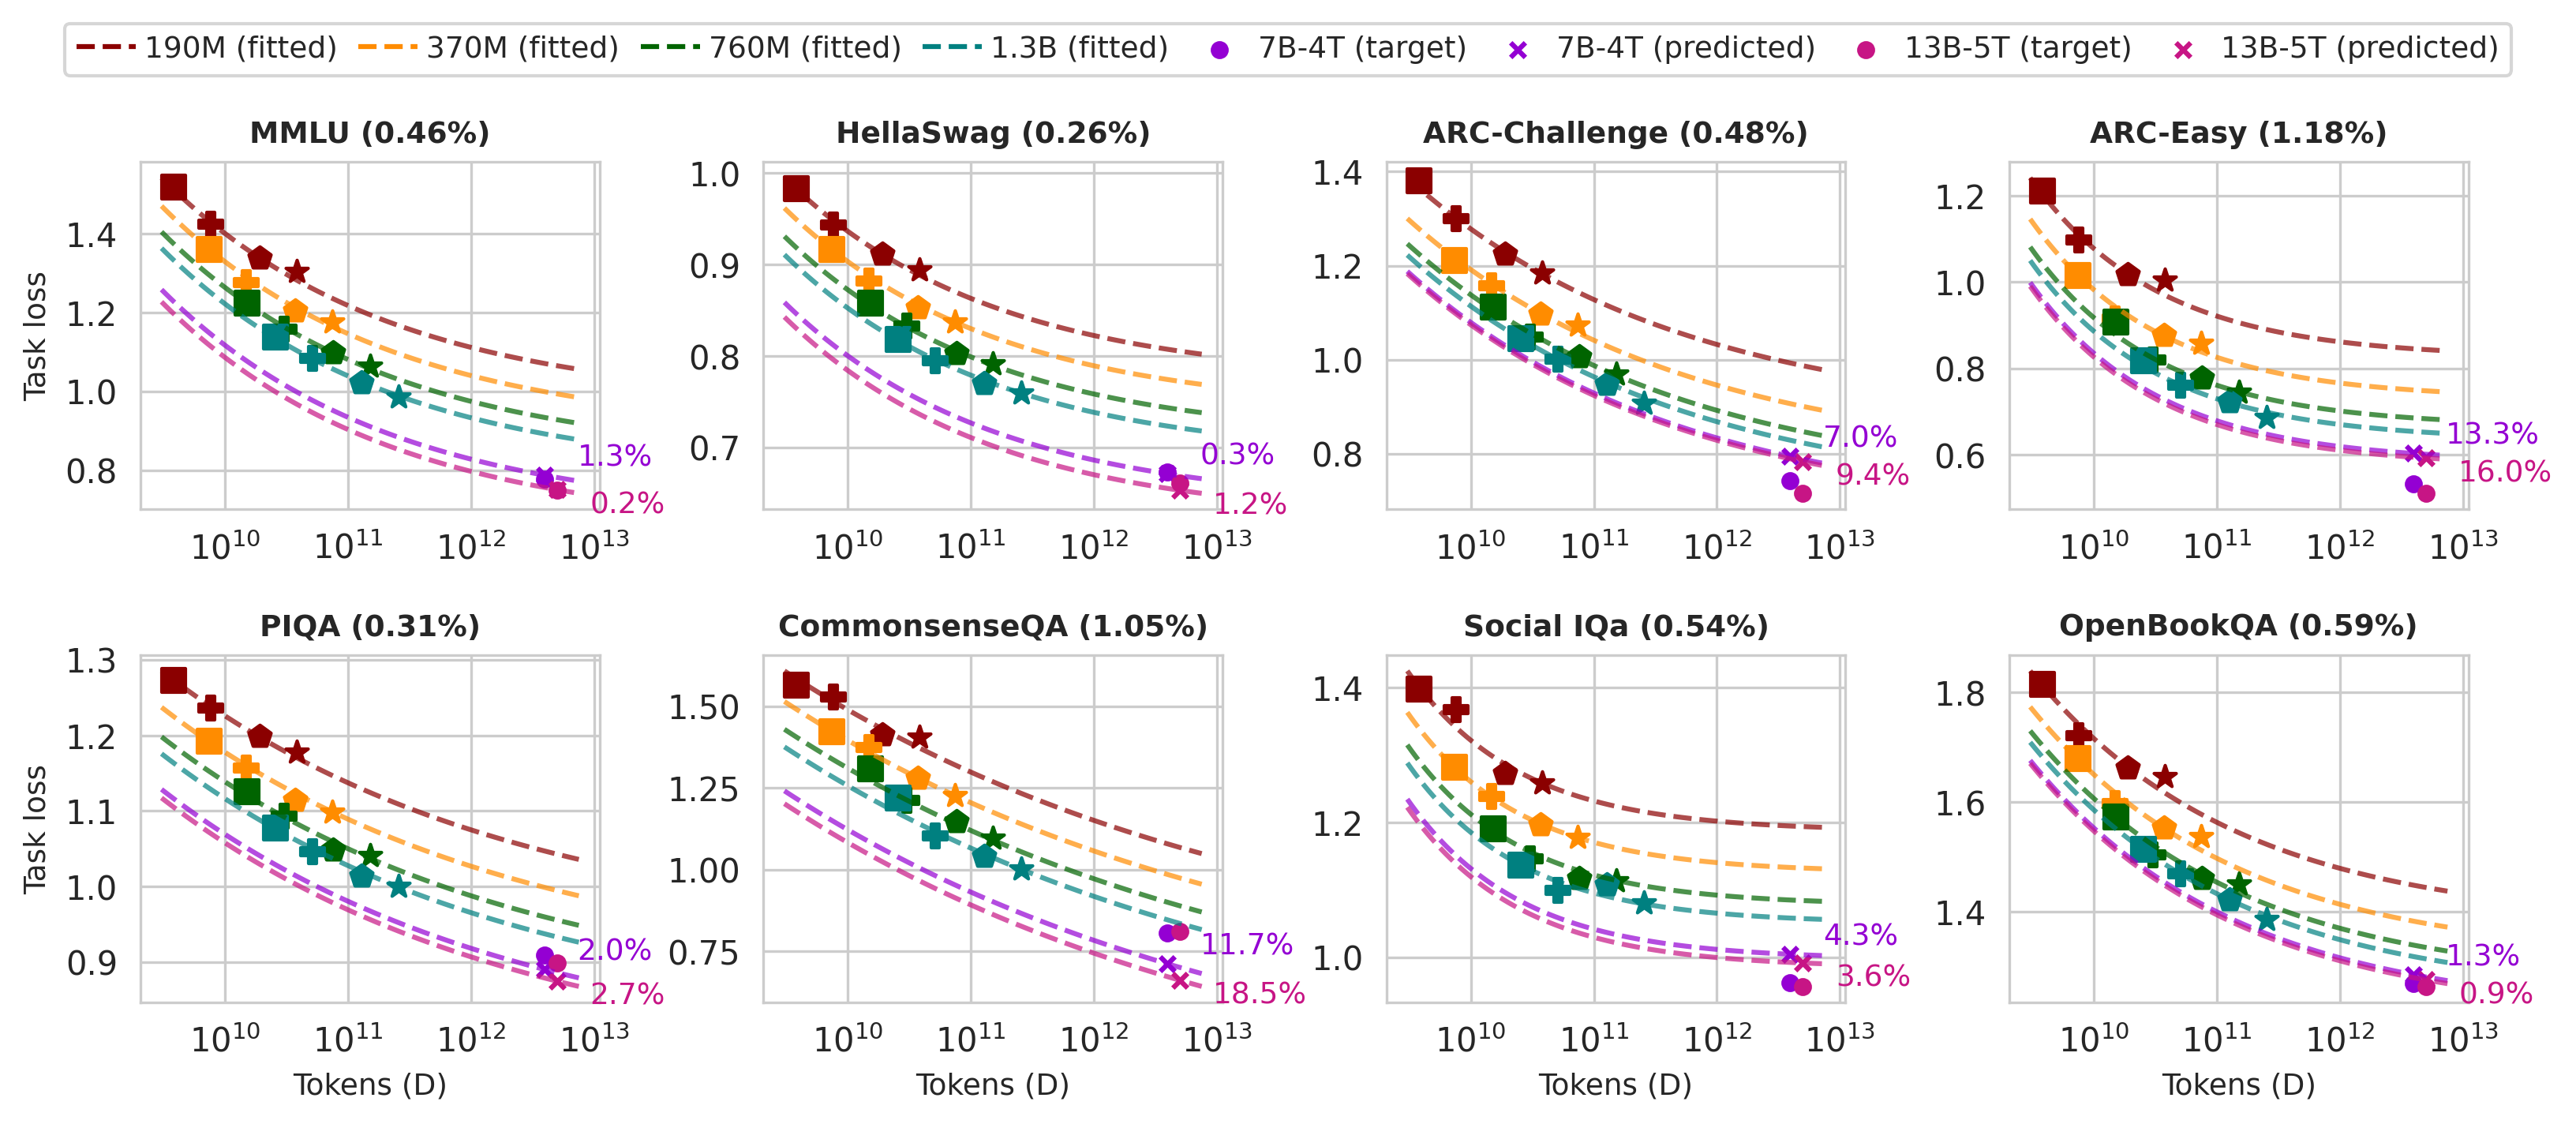
\includegraphics[width=\linewidth]{images/step1_main.png}
\vspace{-16pt}
\caption{
    Task loss vs training scale $(N, D)$, with fitting on the power function in \autoref{eqn:power}.
    \ding{110} = 1xC; \ding{58} = 2xC; $\pentagofill$ = 5xC; $\bigstar$ = 10xC.
    We report the average relative fitting error in parentheses after the task name, and prediction error next to the target model point.
    %In general, the power function fits well to data points from the ladder models, and the fitted function makes rather reliable predictions for the targer models.
    %See \autoref{tab:fitted_params} for the parameters of the fitted functions.
}
\label{fig:step1}
\vspace{-8pt}
\end{figure*}